\documentclass[10pt]{standalone}
\usepackage{amsmath}
\usepackage{pgf,tikz}
\usepackage{mathrsfs}
\usetikzlibrary{arrows}
\pagestyle{empty}

\begin{document}

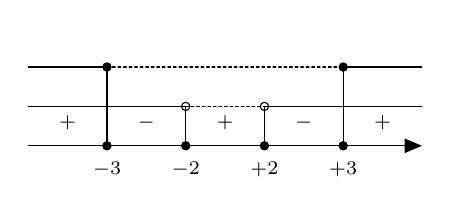
\begin{tikzpicture}[line cap=round,line join=round,>=triangle 45,x=1.0cm,y=1.0cm]

\draw[->] (1,0.) -- (6,0.);

\clip(1,-0.5) rectangle (6,1.5);
\draw  (2.,1.)-- (2.,0.);
\draw  (5.,1.)-- (5.,0.);
\draw  (4.,0.5)-- (4.,0.);
\draw  (3.,0.5)-- (3.,0.);
\draw  (1.,0.5)-- (3.,0.5);
\draw [dash pattern=on 1pt off 1pt] (3.,0.5)-- (4.,0.5);
\draw  (4.,0.5)-- (6.,0.5);
\draw  (1.,1.)-- (2.,1.);
\draw [dash pattern=on 1pt off 1pt] (2.,1.)-- (5.,1.);
\draw  (5.,1.)-- (6.,1.);
\begin{scriptsize}
\draw [fill=black] (2.,0.) circle (1.5pt);
\draw (2.0,-0.3) node {$-3$};
\draw [fill=black] (3.,0.) circle (1.5pt);
\draw (3.0,-0.3) node {$-2$};
\draw [fill=black] (4.,0.) circle (1.5pt);
\draw (4.0,-0.3) node {$+2$};
\draw [fill=black] (5.,0.) circle (1.5pt);
\draw (5.0,-0.3) node {$+3$};
\draw  (3.,0.5) circle (1.5pt);
\draw (4.,0.5) circle (1.5pt);
\draw [fill=black] (2.,1.) circle (1.5pt);
\draw [fill=black] (5.,1.) circle (1.5pt);
\draw (1.5,0.3) node {$+$};
\draw (2.5,0.3) node {$-$};
\draw (3.5,0.3) node {$+$};
\draw (4.5,0.3) node {$-$};
\draw (5.5,0.3) node {$+$};
\end{scriptsize}
\end{tikzpicture}
\end{document}